\section{Scenario's}
De scenario view is een representatie van de belangrijkste use cases van het systeem \parencite{4+1ViewModelPaper}.
De use cases zijn opgesteld door middel van de geprioriteerde lijst van requirements van het onderzoek \parencite{DanteOnderzoek}.
Om de verschillende use cases en interactie met andere actoren in het systeem in beeld te krijgen wordt er gebruik gemaakt van een use case diagram \parencite{UseCaseDiagram}.
In figuur \ref{fig:UseCaseDiagramCMS(1)} \ref{fig:UseCaseDiagramCMS(2)} \ref{fig:UseCaseDiagramBekijkenVanContent} zijn de verschillende use case diagramen te zien.
Er is voor gekozen om de use cases voor het CMS-platform op te delen om het meer overzichtelijk te maken.

\whitespace[2]
\begin{graphic}
	\captionsetup{type=figure}
	\caption{Use case diagram CMS(1)}
	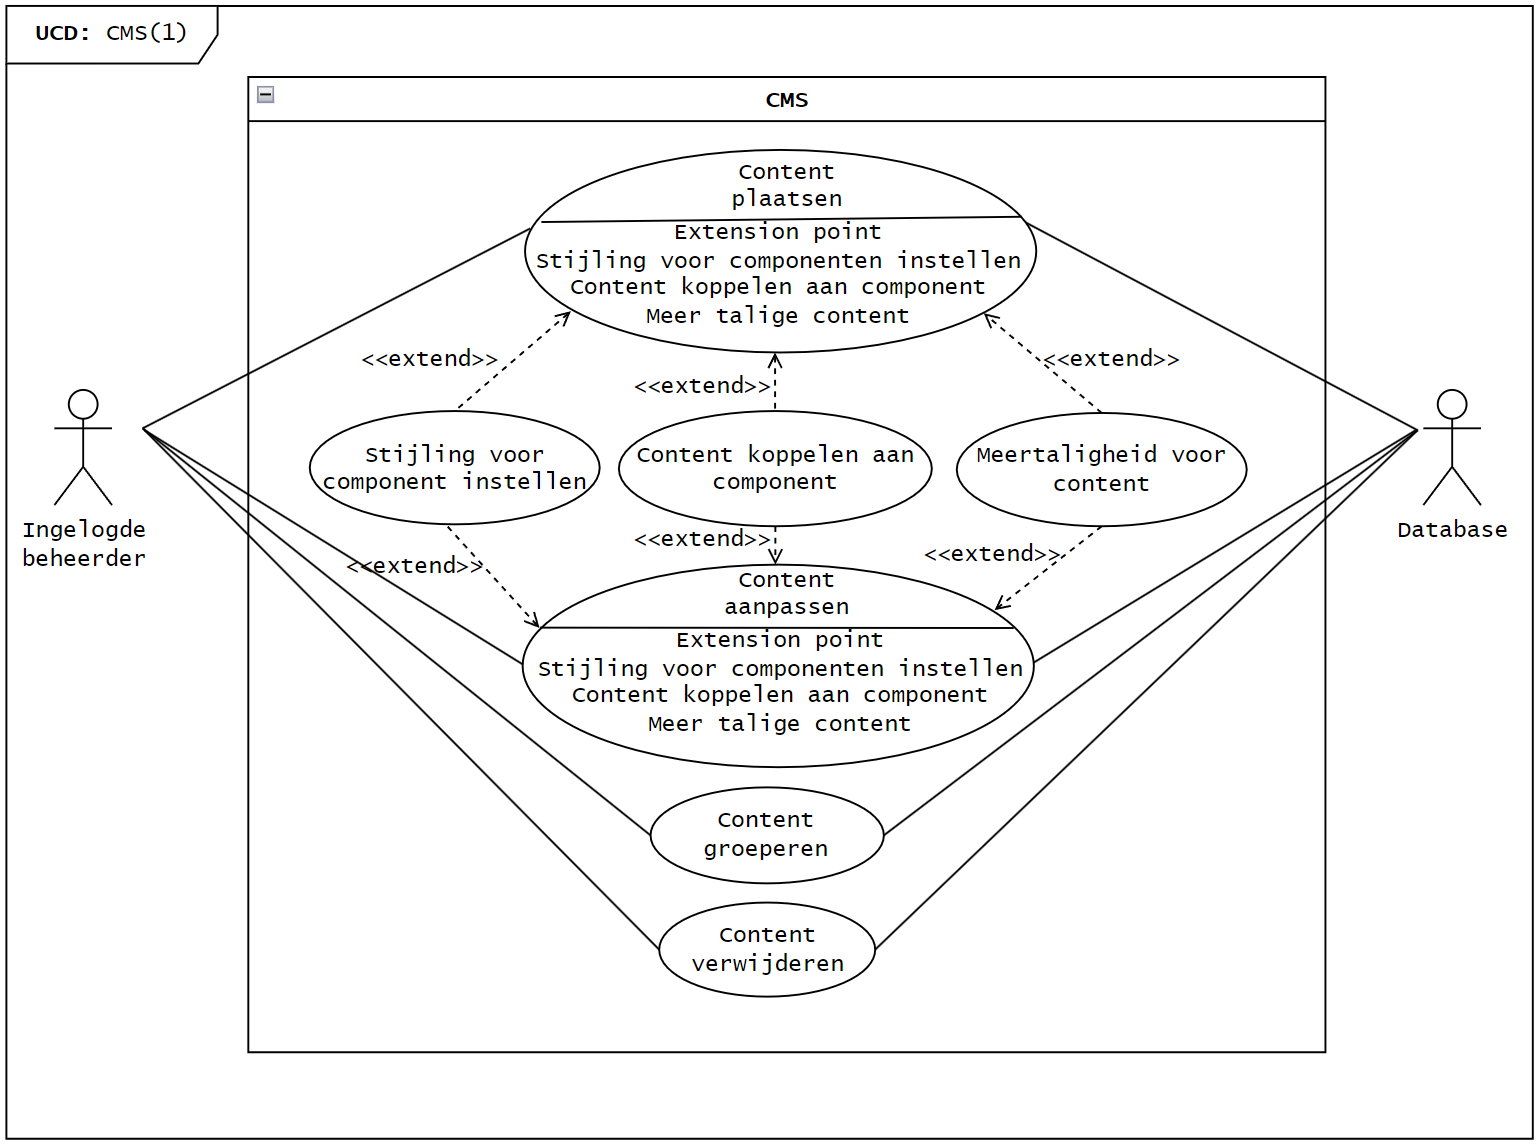
\includegraphics[scale=0.6]{UseCaseDiagramCMS(1).png}
	\label{fig:UseCaseDiagramCMS(1)}
\end{graphic}

\whitespace[2]
In figuur \ref{fig:UseCaseDiagramCMS(1)} zijn de verschillende use cases die te maken hebben met content binnen het CMS.
Content wordt gedefineerd als informatie dat op de site te vinden hierbij kun je denken aan een card, text of een afbeelding.
 
\newpage

\whitespace
Voor de overige functionaliteiten is er in figuur \ref{fig:UseCaseDiagramCMS(2)} ook een use case diagram te vinden.
Dit use case diagram toont het authenticatie en algemene site functionaliteit.

\whitespace
\begin{graphic}
	\captionsetup{type=figure}
	\caption{Use case diagram CMS(2)}
	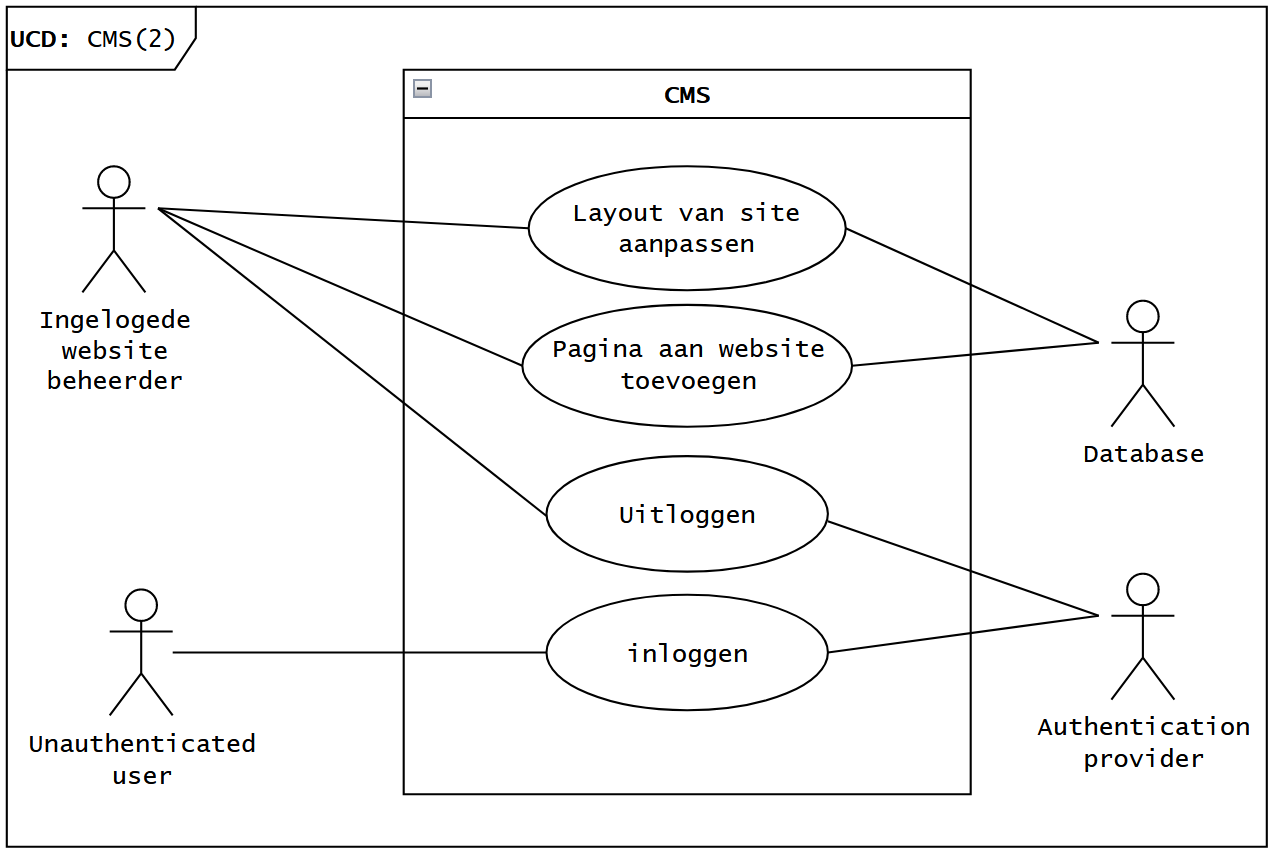
\includegraphics[scale=0.68]{UseCaseDiagramCMS(2).png}
	\label{fig:UseCaseDiagramCMS(2)}
\end{graphic}

\whitespace
Het laatste diagram is gemaakt voor de klanten site.
Dit is de locatie waar de (website) bezoeker de content kan lezen.

\whitespace
\begin{graphic}
	\captionsetup{type=figure}
	\caption{Use case diagram Klant site}
	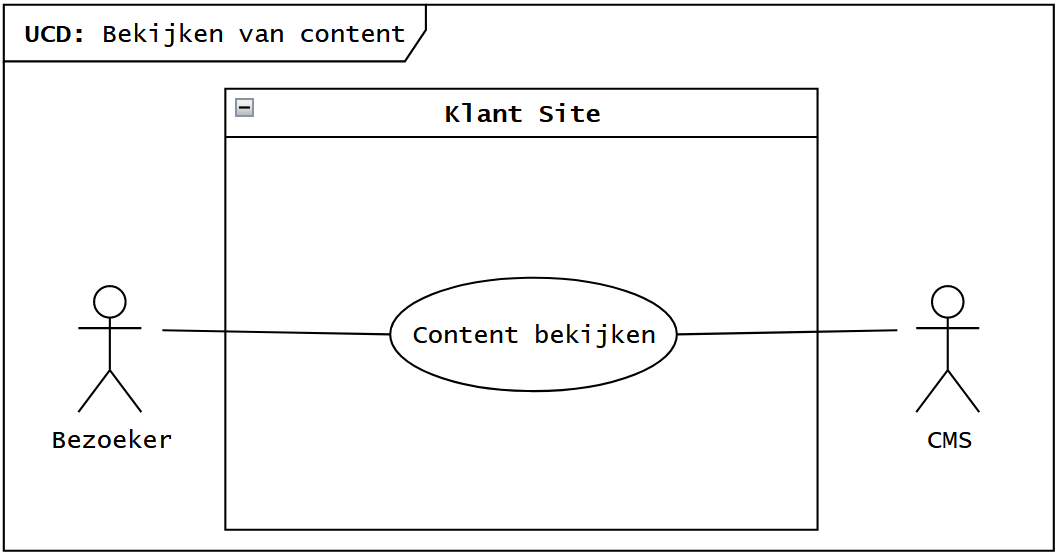
\includegraphics[scale=0.8]{UseCaseDiagramBekijkenVanContent.png}
	\label{fig:UseCaseDiagramBekijkenVanContent}
\end{graphic}
